\setboolean{IsHalfPage}{false}%
\setboolean{IsHalfPageLeftCol}{false}%
\setboolean{IsHalfPageRightCol}{false}%
\def\ChapterTitle{%
	Kemayoran A4B Low-Cost Residences
}
\def\ChapterUrl{%
	https://arnottferels.github.io/work/kemayoran-a4b
}
\def\ChapterDescription{%
	Harmonizing Sustainability and Affordability in Post-COVID Urban Living
}
\def\ChapterDetailsLine{%
	Master's Design Studio 1 -- 2021 | Low-cost Housing Research; Apartment Design; Design Optimization | Central Jakarta, Indonesia}
\def\ChapterDetailsTabular{%
	\begin{tabular}{@{}ll}
		\textbf{Type}     & Individual work                                                                    \\
		\textbf{Software} & Revit, Rhino, Grasshopper, Galapagos, Ladybug Tools, Twinmotion \& Adobe Photoshop \\
		\textbf{Advisor}  & Woerjantari Kartidjo                                                               \\
		\textbf{URL}      & \textcolor{blue}{\footnotesize\texttt{\href{\ChapterUrl}{\ChapterUrl}}}            \\
	\end{tabular}
}
\def\ChapterAbstract{%
	This study aims to create designs for government housing in Kemayoran, Jakarta, specifically for people with lower incomes. The approach is innovative, focusing on changing how buildings are designed. Despite challenges from the COVID-19 pandemic, the project transforms urban areas by combining flexibility and environmental consideration. The design incorporates nature-friendly concepts, including communal green spaces. Tools like the Galapagos Solver are used to shape the exteriors of buildings and adapt interiors based on the weather. The primary focus is on natural cooling and protection from the sun. The research suggests that planning cities this way results in homes that meet current needs and address significant challenges in the future.
}
\def\ChapterFrontmatter{%
	\chapter*{\ChapterTitle}\addcontentsline{toc}{chapter}{\ChapterTitle}
	\ChapterSetTocAddData{\ChapterDetailsLine}
	\ChapterSetDetailsData{\ChapterDescription}{\ChapterDetailsLine}{\ChapterDetailsTabular}
	\RuleAbstract%
	\ChapterAbstract
}
\StartTwoColumnLayout
\ChapterFrontmatter
\vfill
\noindent
\hyphenpenalty=10000
\begin{minipage}[t]{0.55\linewidth}
	\section*{%
	  Issues \& Strategies
	 }
	\begin{table}[H]
	\renewcommand{\arraystretch}{3}
	\RaggedRight
	\small
	\begin{tabularx}{\linewidth}{p{1.5cm} X X}
		\textbf{Period}                      & \textbf{Issues}                                        & \textbf{Strategies}                                                              \\
		\midrule
		COVID-19 pandemic (2020--2021)       & Airborne virus transmission \& Overcrowding prevention & Avoiding dense gatherings and maintaining physical distance                      \\
		\midrule
		Post-pandemic \& future (2022--2045) & Pandemic evolution into endemic state                  & Implementing passive measures for ongoing health considerations                  \\
		\midrule
		Society 5.0 era (2045<)              & Human adaptation to technological advancements and AI  & Integrating smart features aligned with Urban Design Guidelines (UDGL) Kemayoran \\
	\end{tabularx}
\end{table}

	\subsection*{Construction Context}
	\begin{table}[H]
	\renewcommand{\arraystretch}{2.25}
	\RaggedRight
	\small
	\begin{tabularx}{\linewidth}{c X X}
		  & \textbf{Why}                          & \textbf{What's next}            \\
		\midrule
		1 & Understanding low-income residents    & Designs for low-income comfort  \\
		\midrule
		2 & Scarcity of green and communal spaces & Green areas for health          \\
		\midrule
		3 & Impact of the pandemic                & Harmonious green-centric living \\
	\end{tabularx}
\end{table}

\end{minipage}
\hfill
\begin{minipage}[t]{0.4\linewidth}
	\section*{%
	  Concept
	 }
	\begin{figure}[H]
	\centering
	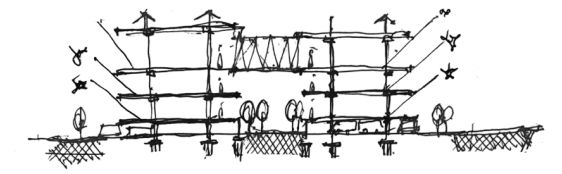
\includegraphics[width=\linewidth]{src/graphics/kemayoran-a4b--concept-sketch.jpg}
	\caption*{%
		\parbox{0.8\linewidth}{%
			\centering
			A green corridor connects Kemayoran A4B and A4A, fostering unity and sustainability.
		}
	}
	\label{
		fig:kemayoran-a4b--concept-sketch
	}
\end{figure}

	\vspace{\baselineskip}%
	\begin{figure}[H]
	\centering
	\includesvg[width=\linewidth]{src/graphics/kemayoran-a4b--concept-mass.svg}
	\label{
		fig:kemayoran-a4b--concept-mass
	}
\end{figure}

\end{minipage}
\vfill
\begin{figure}[H]
	\centering
	\includesvg[width=\linewidth]{src/graphics/kemayoran-a4b--axonometric-context.svg}
	\label{
		fig:kemayoran-a4b--axonometric-context
	}
\end{figure}

\columnbreak%
\section*{%
  Optimization
 }
\begin{center}
	\noindent
	\begin{minipage}[t]{0.55\linewidth}
		\begin{figure}[H]
	\centering
	\includesvg[width=\linewidth]{src/graphics/kemayoran-a4b--optimization.svg}
	\label{
		fig:kemayoran-a4b--optimization
	}
\end{figure}

	\end{minipage}%
	\hfill
	\begin{minipage}[t]{0.4\linewidth}
		In response to challenges posed by the COVID-19 pandemic, the architecture prioritizes adaptability. By using tools like the Galapagos Solver, the project strategically adjusts external appearances and spatial arrangements to facilitate natural cooling and protect against radiation, promoting sustainability.
		\vspace{\baselineskip}%
		\newline%
		Upon evaluating both designs, Iteration A emerges as the preferred solution. Achieving a~$14^\circ$ rotation from North in 38~minutes and 21~seconds, it records an annual solar radiation of 18.723~million~$\text{kWh/m}^2$ (a 5.83\% increase from Iteration B). Despite a double-loaded design and relying on the Vertical Pocket system for tower comfort, Iteration A excels in floor efficiency for the targeted 3{,}000 population, obtaining the lowest ASR ranking.
		\vspace{\baselineskip}%
		\newline%
		On the other hand, Iteration B, completed in 38~minutes and 20~seconds, adopts a 14° angle from North, resulting in an ASR of 17.630~million~$\text{kWh/m}^2$. While maintaining the lowest ASR rank and providing more open spaces, it compromises on floor efficiency above the refuge floor and relies on the Vertical Pocket system for the comfort of the 3000-person target.
	\end{minipage}
\end{center}
\section*{%
  Features
 }
\begin{center}
	\begin{minipage}{0.8\linewidth}
		\begin{figure}[H]
	\centering
	\includesvg[width=\linewidth]{src/graphics/kemayoran-a4b--features.svg}
	\label{
		fig:kemayoran-a4b--features
	}
\end{figure}

	\end{minipage}
\end{center}
\section*{%
  Design
 }
\begin{figure}[H]
	\centering
	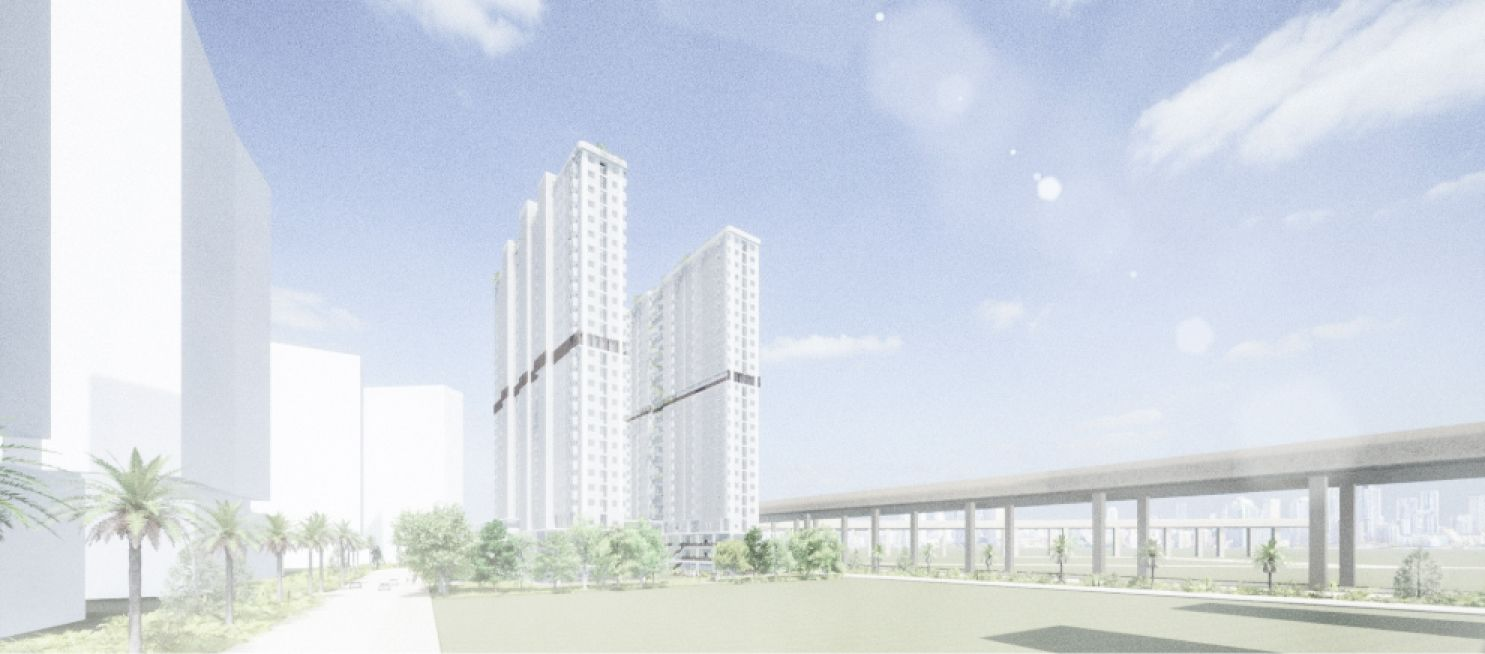
\includegraphics[width=0.9\linewidth]{src/graphics/kemayoran-a4b--design.jpg}
	\caption*{%
		The perspective at eye level from the road towards Kemayoran A4B.
	}
	\label{
		fig:kemayoran-a4b--design
	}
\end{figure}

\EndTwoColumnLayout
\begin{minipage}[t]{0.3\linewidth}
	\section*{%
	  Features
	 }
	\begin{figure}[H]
	\centering
	\includesvg[width=0.8\linewidth]{src/graphics/kemayoran-a4b--axonometric.svg}
	\caption*{%
		Axonometric view illustrating the distribution of facilities across different floors in the building.
	}
	\label{
		fig:kemayoran-a4b--axonometric
	}
\end{figure}
%
\end{minipage}%
\hfill
\begin{minipage}[t]{0.7\linewidth}
	\section*{%
	  Unit config
	 }
	\begin{figure}[H]
	\centering
	\includesvg[width=\linewidth]{src/graphics/kemayoran-a4b--unit-config.svg}
	\label{
		fig:kemayoran-a4b--unit-config
	}
\end{figure}

	\vspace{0.5cm}%
	\small
	\setlength{\columnsep}{0.75cm}
	\begin{multicols}{3}
		In this design, various plans have been employed to accommodate different living spaces for different needs. The Standard Studio (18~$\text{m}^2$) designed for one person can be expanded into a larger Two-Bedroom (36~$\text{m}^2$) and further to a spacious Corner Three-Bedroom (54~$\text{m}^2$). Shared areas promote a sense of community among neighbors, while well-planned paths facilitate easy movement.
		\newline%
		Moreover, the design focuses on inclusivity and utility, offering both small and large apartments with attractive views. Accessible options, such as the Accessible Studio (36~$\text{m}^2$) and Corner Accessible Studio (36~$\text{m}^2$), are integrated to cater to a diverse range of residents.
	\end{multicols}
	\section*{%
	  Drawing
	 }
	\begin{figure}[H]
	\centering
	\includesvg[width=\linewidth]{src/graphics/kemayoran-a4b--drawing.svg}
	\label{
		fig:kemayoran-a4b--drawing
	}
\end{figure}

\end{minipage}
\newpage
